%-------database
\section*{Connessione e script database}
Durante la fase di sviluppo dell'applicazione, per connettersi al database remoto è stato necessario, per motivi di sicurezza, eseguire un tunneling SSH tramite il comando da terminale: 
\begin{lstlisting}
ssh -L localport:host:hostport user@ssh_server -N 
\end{lstlisting}
Lo script \emph{database.sql} usato per creare il database si trova nella directory \emph{AuleProjSVGWT/src} come mostrato in figura \ref{fig:dbSQL}.

\begin{figure}[!htb]
\centering%
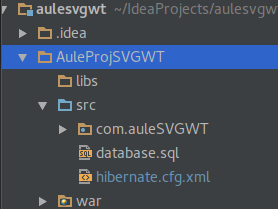
\includegraphics[scale=0.5]{screenSQL.png}%
\caption{Cartella contenente script del database.}\label{fig:dbSQL}%
\end{figure}

\FloatBarrier
\section*{Creazione mappe e colorazione}
Le piantine dei locali universitari non possono essere inserite direttamente nel server perch\`e sono in un formato che non \`e compatibile col programma.Lo scopo di questa appendice \`e quello di spiegare la procedura da seguire per  ottenere dei file adeguati alle funzionalit\`a dell'applicazione.\\\\Le immagini fornite dal dipartimento sono in formato \textit{dwg}, quindi la prima operazione da effettuare \`e quella di convertirle in \textit{svg} e salvarle con questo nome: "\textit{nome\_edificio-numero\_piano.svg}".In rete esistono diversi software che consentono di cambiare l'estensione del file, nel nostro caso \`e stato utilizzato AIGraph CAD Viewer(versione 3.3.1 o superiore).Un altro metodo consiste nel trasformare i file \textit{dwg} in \textit{dxf}, importarli su Inkscape, per poi salvarli come \textit{svg}.Tra le due alternative \`e stata adottata la prima perch\`e ha permesso di generare figure con una migliore qualit\`a grafica.\\\\Nel file ottenuto le stanze non sono ancora elementi grafici indipendenti, perci\`o se si vogliono gestire eventi su ognuna di esse \`e necessario inserire, all'interno del file, delle forme geometriche che le racchiudano.Questa operazione, molto onerosa in termini di tempo, pu\`o essere velocizzata se si utilizza Inkscape.Le forme geometriche inserite con questo tool devono essere di tipo \textit{"rect"} o \textit{"path"}, il motivo di questa operazione sar\`a trattato nella parte in cui si parla del codice Java.Dopo aver creato il profilo di una stanza bisogna selezionare l'opzione \textit{object properties}(come avviene in figura \textbf{\ref{fig:TUT_ink}}) e introdurre nei tre riquadri disponibili la stringa 
\\
"\textit{nome\_edificio-numero\_piano-numero\_stanza}": l'inserimento di questi parametri, in particolar modo dell'ID, servir\`a al software per risalire alla stanza.Questo perch\`e i singoli termini della stringa hanno una corrispondenza con i dati inseriti nel database:  \\
\textit{nome\_edificio} \`e associato a \textit{building\_name} della tabella "building", invece \textit{numero\_piano} e \textit{numero\_stanza} equivalgono a \textit{room\_floor} e \textit{room\_number} della tabella "room".Dato che la loro combinazione rappresenta un'\textit{UNIQUE KEY} \`e possibile sfruttarla per risalire ad un unica istanza di "room".
\begin{figure}[H]
\centering
\fbox{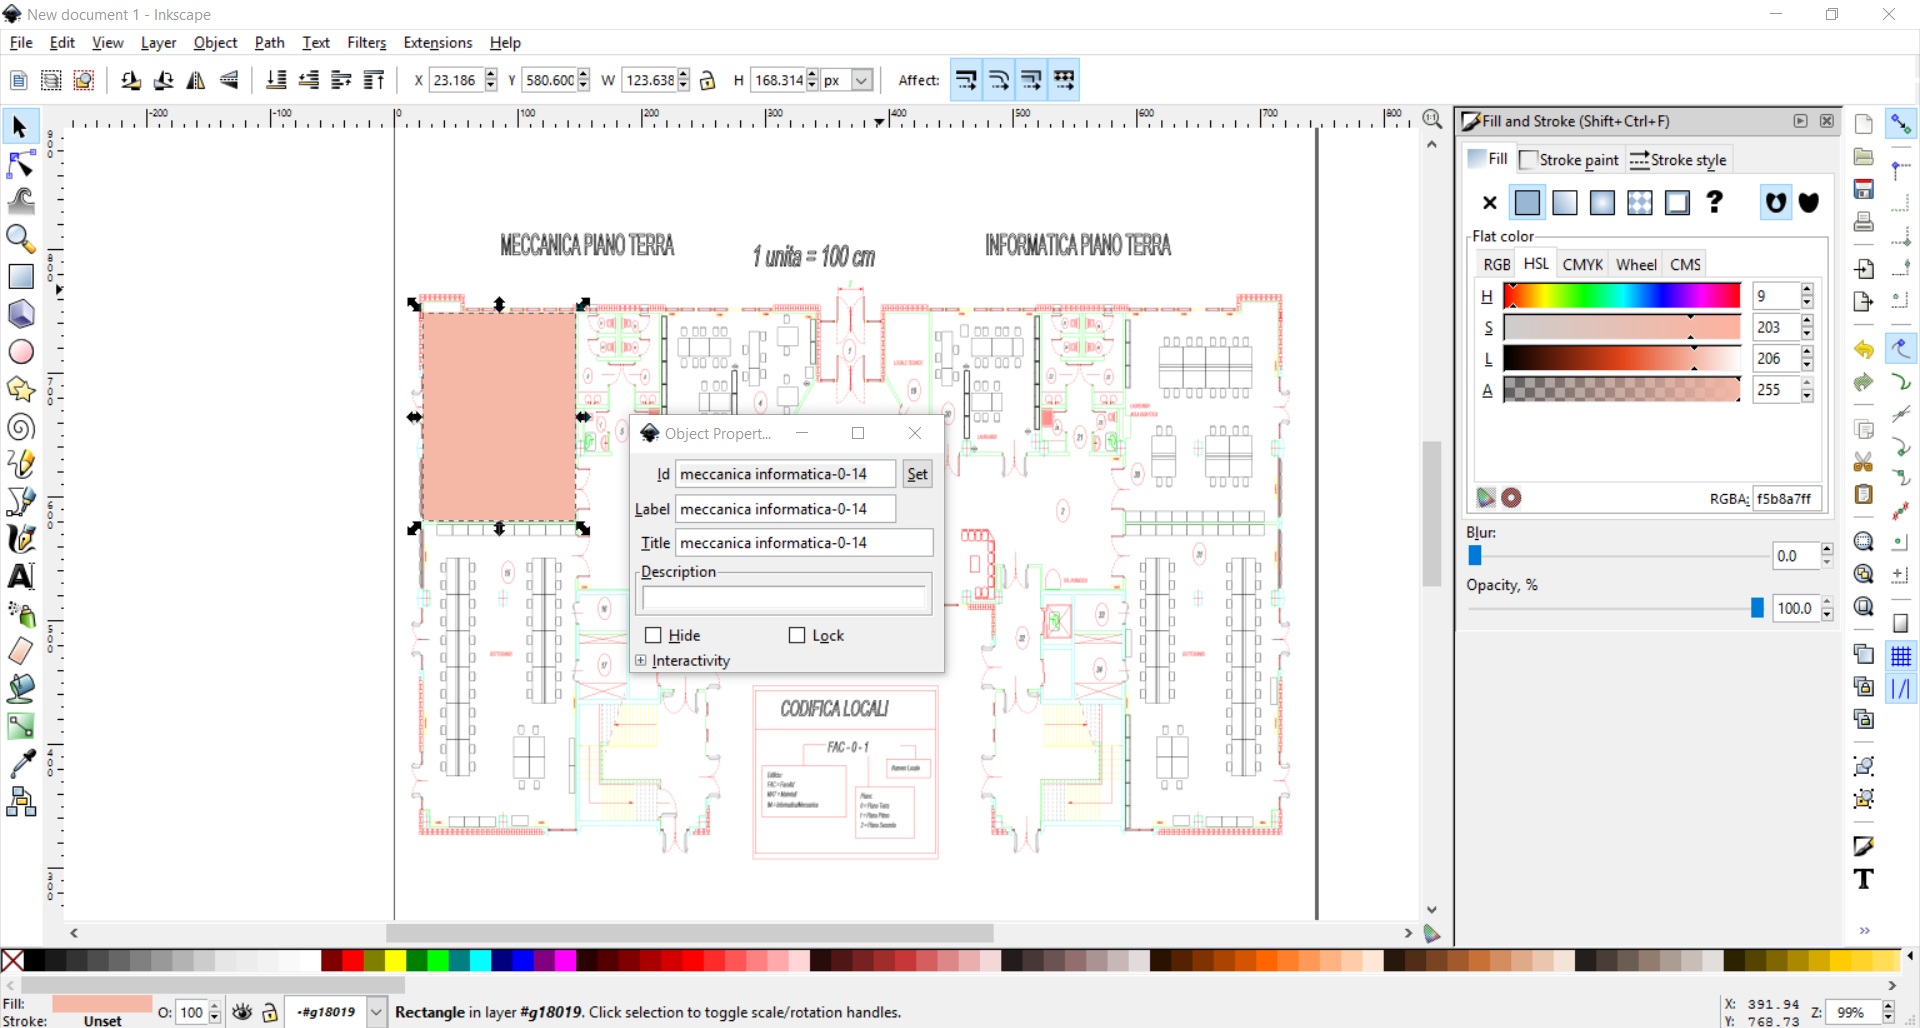
\includegraphics[width=150mm,height=85mm]{esempioInkscape.png}}
\caption{Inkscape: inserimento stanza cliccabile}
\label{fig:TUT_ink}%
\end{figure}
\noindent\\Infine \`e necessario un ultimo passaggio: con un editor di testo o con un IDE qualsiasi(con \textit{encodig:"UTF-8"}) devono essere modificate e inserite alcune stringhe nel file.Per prima cosa bisogna controllare che siano presenti i seguenti attributi all'interno del tag \textit{<svg>}.
\begin{lstlisting}
<?xml version="1.0" encoding="UTF-8" standalone="no"?>
<svg
	..
	xmlns:dc="http://purl.org/dc/elements/1.1/"
	..
	xmlns:svg="http://www.w3.org/2000/svg"
	xmlns="http://www.w3.org/2000/svg"
	..
	version="1.1"
	..
	sodipodi:docname="materiali-1.svg"
\end{lstlisting}
\`E fondamentale che sia inserito anche all'interno il nome del file, e che la versione dello \textit{standard} sia la "\textbf{1.1}".\\Se non vengono rispettati questi dettagli possono insorgere degli errori nelle librerie che lavorano con le immagini.\\Di seguito \`e riportato un esempio di come deve apparire il codice di una stanza.
\subsubsection*{ANDROID}
\begin{lstlisting}
<path
   style="fill:none;stroke:none;fill-opacity:0.5;stroke-width:0.99871397px;
   stroke-linecap:butt;stroke-linejoin:miter"
   d="m 247.97113,203.91145 -10.22383,
   -88.12825 -37.94946,5.39561 10.5704,87.76853 z"
   id="materiali-1-4"
   inkscape:connector-curvature="0"
   inkscape:label="materiali-1-4"><title
     id="title30939">materiali-1-4</title>
</path>
\end{lstlisting}
Le stringhe \textbf{"fill:none"},\textbf{"stroke:none"} e \textbf{"fill-opacity:0.5"} devono sempre essere presenti tra le prorpiet\`a di \textit{style}, senza queste non sarebbe possibile effettuare la colorazione.Gli altri attributi invece possono essere trascurati, l'unica eccezione si ha per quelli che contengono la parola \textit{"gradient"}, in questo caso \`e consigliabile eliminarli perch\`e potrebbero creare delle sfumature nel colore.\\Come \`e stato detto in precedenza il codice relativo ad un stanza deve essere contenuto in elementi di tipo \textit{<path>} o \textit{<rect>}, se ne vengono utilizzati altri \`e necessario riadattare anche la parte Java.
\subsubsection*{GWT}
Va precisato che le librerie usate per GWT non supportano l'attributo \textbf{"none"}, dunque, essendo il numero di immagini limitato e la loro dimensione contenuta, si \`e deciso di utilizzare due file indipendenti per ogni ogni piantina: uno per Android nella cartella \textit{res/ImageAndroid} e uno per GWT nella cartella \textit{res/ImageGWT}.Di seguito \`e mostrato il codice riadattato per GWT.
\begin{lstlisting}
<path
   style="fill:transparent;stroke:transparent;
   fill-opacity:0.5;stroke-width:0.99871397px;
   stroke-linecap:butt;stroke-linejoin:miter"
   d="m 247.97113,203.91145 -10.22383,-88.12825 -37.94946,
   5.39561 10.5704,87.76853 z"
   id="materiali-1-4"
   inkscape:connector-curvature="0"
   inkscape:label="materiali-1-4"><title
   id="title30939">materiali-1-4</title>
</path> 
\end{lstlisting}
Come si pu\`o notare l'unica differenza sta nella sostituzione di \textit{none} con \textit{transparent}.
\subsubsection*{CODICE JAVA}
In questa sezione vengono analizzate le parti di codice Java che servono per effettuare lavorare sulle immagini.Nel primo riquadro \`e esposto il metodo con cui ottenere la lista delle stanze all'interno di una piantina.\\Grazie alla stringa \textit{"NOME\_FILE"} \`e possibile sapere su quale file effettuare la ricerca.\\Se si osserva attentamente, nelle righe 9-10, si pu\`o notare che l'indagine avviene solo per elementi di tipo "path" e "rect", nel caso venissero usate altre forme geometriche \`e necessario aggiungerle in questa zona del codice. 
\begin{lstlisting}
String fullPath = servletContext.getRealPath(path);
URI uri = new File(fullPath+"/" + NOME_FILE + ".svg").toURI();
SVGMetaPost converter;
ArrayList<String> room = new ArrayList<>();
	try{
    	converter = new SVGMetaPost(uri.toString());
    	Document doc = converter.getSVGDocument();
    
    	NodeList n = doc.getElementsByTagName("rect");
    	NodeList p = doc.getElementsByTagName("path");
    	for(int i =0 ;i<n.getLength();i++){
    		if(((Element) n.item(i)).getAttribute("id").contains(NOME_FILE)){
            	        room.add(((Element) n.item(i)).getAttribute("id"));
			}
		}
    	for(int i =0 ;i<p.getLength();i++) {
    		if(((Element) p.item(i)).getAttribute("id").contains(NOME_FILE)){
    			room.add(((Element) p.item(i)).getAttribute("id"));
    		}
    	}
	}catch (IOException e){
		e.printStackTrace();
	}		
	
return room;

}
\end{lstlisting}
\noindent\\Nella seconda area viene presentato lo pseudocodice per ottenere la variazione dei colori nelle piantine. 
\begin{lstlisting}
per ogni stanza{
	sum = somma dei pesi dei ruoli di ogni persona che occupa la stanza;
	dim = la dimensione in metri quadri della stanza;

	if ( dim == 0 e sum != 0 ){
		//colora la stanza di ROSSO;
	}
	else if( dim == sum e dim != 0 ){
		//colora la stanza di VERDE;
	}
	else if( sum > dim e dim != 0 ){
		//colora la stanza con una gradazione di ROSSO
	}
	} else if (sum < dim e dim != 0 ){
		//colora la stanza con una gradazione di BLU
	}

}
\end{lstlisting}
Per avere le gamme di ROSSO e BLU si opera in questo modo:
\\\textbf{Spazio disponibile superato}\\Si effettua questa divisione tra \textit{dim} e \textit{sum}.Il numero che otteniamo, compreso tra 0 e 1, viene moltiplicato per 200 e trasformato in numero esadecimale.Il valore esadecimale viene poi usato per creare una stringa che identifichi il colore.
\begin{lstlisting}
Double valued = ((double) dim / sum) * 200;
Integer value = valued.intValue();
String color = "#FF"+Integer.toHexString(value)+Integer.toHexString(value);
\end{lstlisting}
In questo modo pi\`u \`e piccolo il rapporto maggiore sar\`a l'intensit\`a del rosso.Non \`e stata sfruttata tutta la gamma di colori del modello RGB,questo perch\`e con numeri compresi tra 200 e 255 si ottengono colorazioni troppo vicine al bianco.
\\\textbf{Spazio disponibile non superato}\\Il funzionamento in questo caso \`e lo stesso, vengono solamente invertiti il rapporto e l' ordine della stringa.
\begin{lstlisting}
Double valued = ((double) sum / dim) * 200;
Integer value = valued.intValue();
String color = "#"+Integer.toHexString(value)+Integer.toHexString(value)+"FF";
\end{lstlisting}
Una volta ottenuto il colore basta andarlo a sostituire nel \textit{fill} della stanza.
Il codice usato per la colorazione delle stanze \`e localizzato in due zone differenti: quello usato dall'app Android si trova nella classe \textit{ImageHandling}(package com.auleSVGWT.server), mentre il codice relativo all Web app si trova nella classe\\ \textit{ShowFloorPresenter}(package com.auleSVGWT.client.presenter), pronto a diventare Javascript dopo la compilazione.


